\documentclass[letterpaper,12pt]{article}
\usepackage{graphicx}
\author{Ryan Nish, Marissa Melen, Victor Aw}
\title{COMP 188 Computer Science Senior Project\\ Fables of
  Sylvus$^{\small \copyright}$ Monster Minder}
\date{2013-11-13}
\begin{document}

\maketitle
\pagebreak
\section{Contributions}
Features list - All team members contributed equally
\pagebreak
\tableofcontents
\pagebreak
\section{Interaction Diagrams}
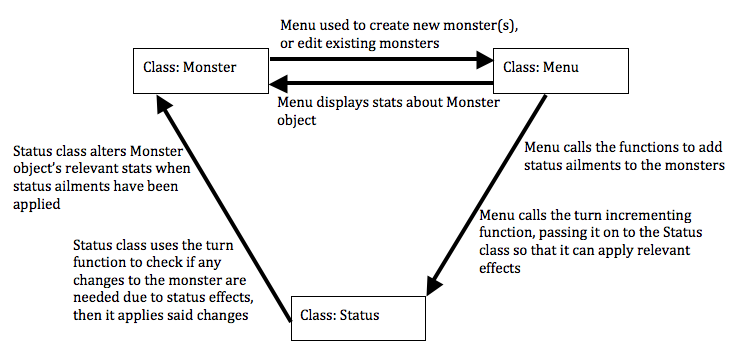
\includegraphics[width=6in]{Class Interaction.png}
\pagebreak
\section{Class Diagrams and Interaction Specifications}
\subsection{Class Diagrams}
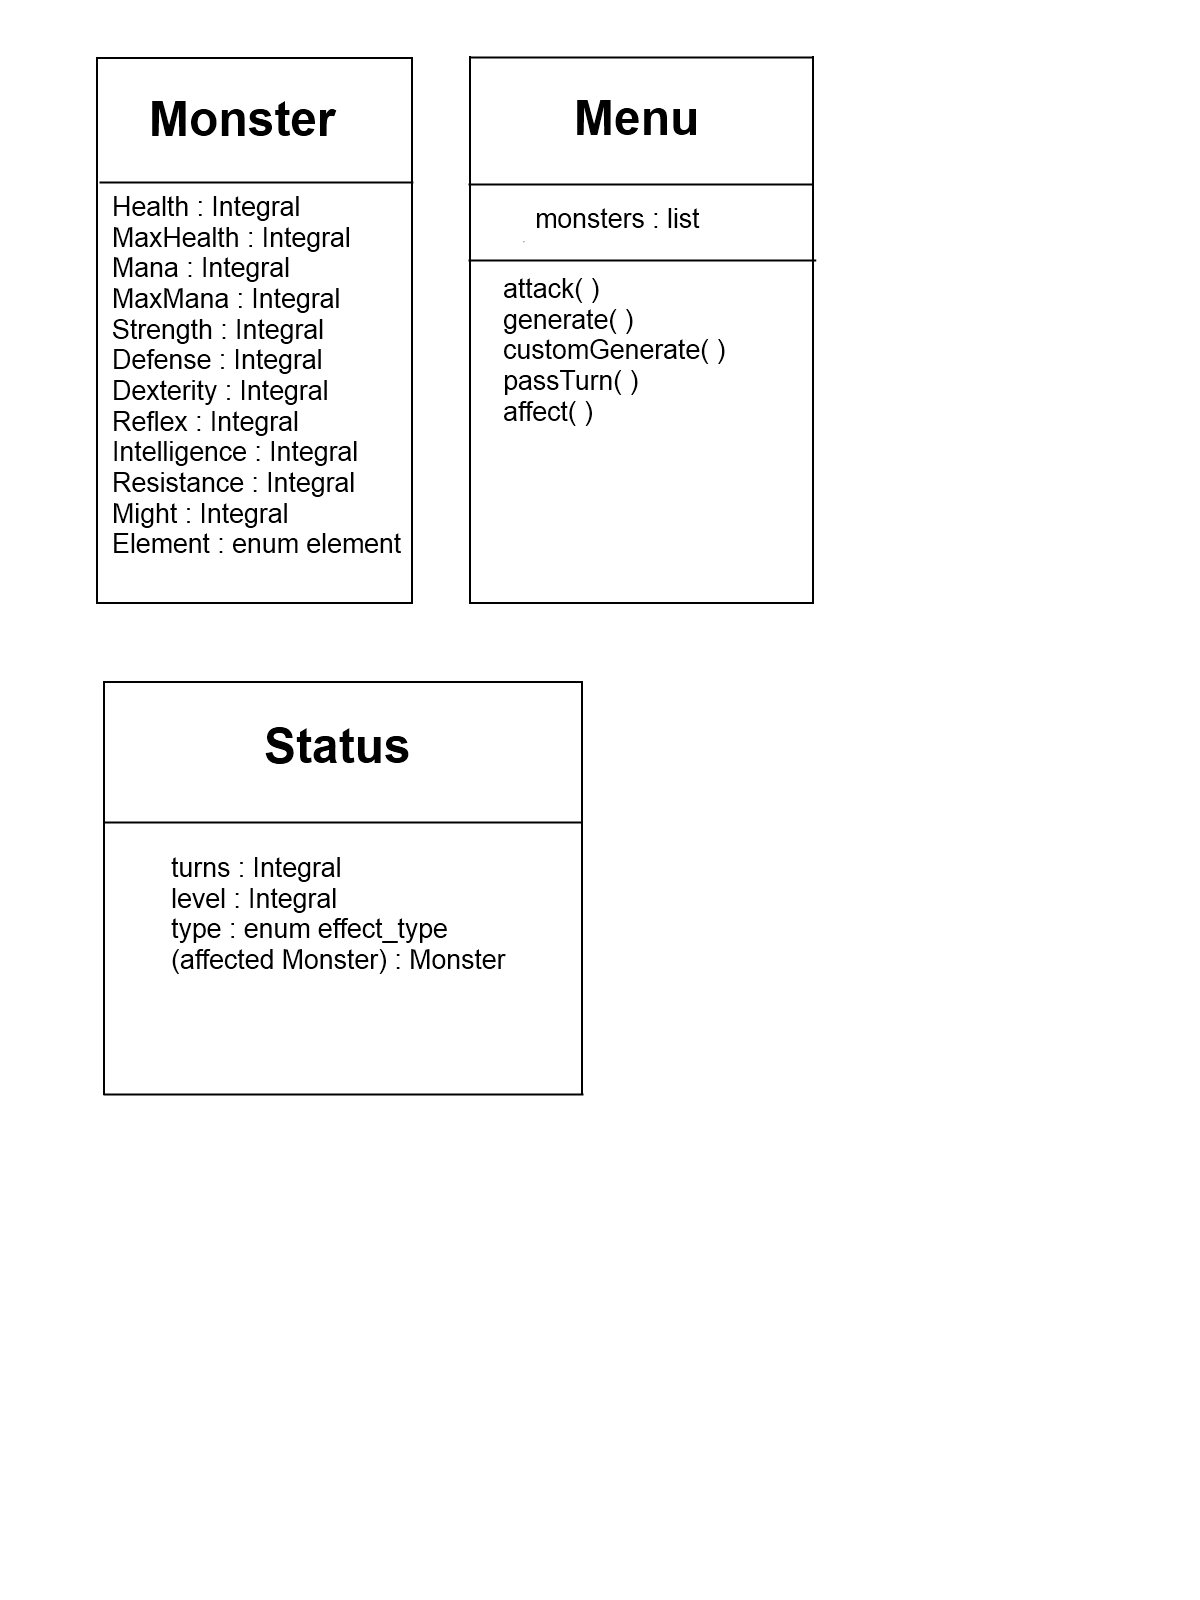
\includegraphics[width=6in]{Class Diagrams.png}
\subsection{Interface Specifications}
\subsubsection{Monster}
\hrulefill
Health : Integral\\
MaxHealth : Integral\\
Mana : Integral\\
MaxMana : Integral\\
Strength : Integral\\
Defense : Integral\\
Dexterity : Integral\\
Reflex : Integral\\
Intelligence : Integral\\
Resistance : Integral\\
Might : Integral\\
Element : enum element\\
\subsubsection{Menu}
monsters : list\\
\hrulefill\\
attack()\\
generate()\\
customGenerate()\\
passTurn()\\
affect()\\
\subsubsection{status}
turns : Integral\\
level : Integral\\
type : enum effect\_type\\
\hrulefill\\
(affected Monster) : Monster\\
\section{System Architecture and Design}
\subsection{Hardware Mapping}
Our system runs on only one machine
\subsection{Network Protocols}
Our system does not use the network
\subsection{System Requirements}
At a bare minimum our system could run on a computer with only an
80x25 terminal and minimal storage space, CPU, and RAM. However, our
system would work much better on a system with a graphical display at
a resolution the user is comfortable with.
\section{Algorithms and Data Structures}
\subsection{Algorithms}
Our project does not use any complex algorithms.
\subsection{Data structures}
First, our system will use a list-like structure, which may, for
example, be a c++ vector. This was chosen because there is not need to
order the data, but that its size cannot be known in advance, and so
an expandable structure is needed. In addition, we will use functions
to update the monsters as they are created, since all monsters will
be created at level 1, and will need to be upgraded to a higher level.\\
\hfill\\

We will also be using a functor, or mutable function, to represent
status ailments and effects, because these by nature modify monsters, however
we still need to have data associated with them, such as level, turns
remaining, and the like.
\section{User Interface Design}
\subsection{Basic Functions}
Our user, the Game Master or GM, will use an interface that will have some 
basic functionality, such as the ability to input the number of players, 
and their average level so that the program can generate an appropriate number 
of monsters at an acceptable level.  In addition, a monster can be selected 
as the target of an attack, and a menu will allow the choosing of the attack type 
(magic or physical), the weapon used (axe, spear, ect) the value the player 
rolled (this affects whether the weapon misses, grazes, or crits), and any 
additional effects that might happen.  Such as weapon specific chances of
status ailments or double strike.  The monster menu will also allow the user to
change the monster's stats directly, if such a need arises via player-specific
ability or GM intervention.  This menu will also facilitate the use of monster
spells.  Since monsters have their own spells, it is up to the GM to decide when
they are used, and the menu will in turn make the necesary changes to monster
mana or other stats.
\section{Plan of Work}
\section{References}
\end{document}



